\documentclass[11pt]{article}
\usepackage{amsthm,amsmath,amssymb,bbm,bm}
\usepackage{mathtools}
\usepackage{natbib}
\usepackage{multirow}
\usepackage[pdftex]{graphicx}
\usepackage{subfigure}
\usepackage{wrapfig}
\usepackage{array}
\usepackage{url}
\usepackage{algorithm}
\usepackage[noend]{algpseudocode}
\usepackage{mathrsfs}
\usepackage{dsfont}
\usepackage{titling}
\usepackage{relsize}
\usepackage{rotating}
\usepackage{enumitem}
\usepackage{booktabs}
\usepackage[usenames,dvipsnames,svgnames,table]{xcolor}
\usepackage[colorlinks=true,
            linkcolor=red,
            anchorcolor=blue,
            citecolor=blue,
            urlcolor=blue]{hyperref}

\usepackage[a4paper,
 %total={170mm,257mm},
 left=28mm,
 top=30mm]{geometry}

\renewcommand{\baselinestretch}{1.1}
{\textwidth=6in}

\usepackage{chngcntr}

\counterwithin{equation}{section}
\theoremstyle{definition}
\newtheorem{definition}{Definition}[section]

\newtheorem{thm}{Theorem}
\newtheorem{lemma}{Lemma}
\counterwithin{thm}{section}
\newtheorem{rmk}{Remark}[thm]
\counterwithin{rmk}{section}
\newtheorem{assump}{Assumption}
\renewcommand\theassump{A\arabic{assump}}


\def\bal#1\eal{\begin{align}#1\end{align}}
\def\balnn#1\ealnn{\begin{align*}#1\end{align*}}

% optimization
\DeclareMathOperator*{\argmin}{arg\,min}
\DeclareMathOperator*{\argmax}{arg\,max}

% various delimiters / bracketing operations
\DeclarePairedDelimiter\parentheses{\lparen}{\rparen}
\DeclarePairedDelimiter\brackets{\lbrack}{\rbrack}
\DeclarePairedDelimiter\set{\{}{\}}
\DeclarePairedDelimiterX{\norm}[1]{\lVert}{\rVert}{#1}
\DeclarePairedDelimiterX{\abs}[1]{\lvert}{\rvert}{#1}
\newcommand{\spn}[1]{\text{span}\parentheses*{#1}}

% expectation bracketing
\DeclarePairedDelimiterX{\expectarg}[1]{[}{]}{%
    \ifnum\currentgrouptype=16 \else\begingroup\fi
    \activatebar#1
    \ifnum\currentgrouptype=16 \else\endgroup\fi
}

% variance bracketing
\DeclarePairedDelimiterX{\variancearg}[1]{(}{)}{%
    \ifnum\currentgrouptype=16 \else\begingroup\fi
    \activatebar#1
    \ifnum\currentgrouptype=16 \else\endgroup\fi
}

% conditional bar conditional expectation / variance
\newcommand{\innermid}{\nonscript\;\delimsize\vert\nonscript\;}
\newcommand{\activatebar}{%
    \begingroup\lccode`\~=`\|
    \lowercase{\endgroup\let~}\innermid
    \mathcode`|=\string"8000
}

% probability
\newcommand{\Prob}{P \, \variancearg}
\newcommand{\E}{\mathbb{E} \, \expectarg}
\newcommand{\Var}{\operatorname{Var}\variancearg}
\newcommand{\Cov}{\operatorname{Cov}\variancearg}
\newcommand\independent{\protect\mathpalette{\protect\independenT}{\perp}}

% indicator function
\def\mOne{{\mathbbm{1}}}
\newcommand{\ind}[1]{\mOne_{\{#1\}}}
\newcommand{\indc}[1]{\mOne_{\{#1\}^c}}

% linear algebra
\newcommand{\Reals}[1]{\mathbb{R}^{#1}}

% dataset
\newcommand{\dataset}{\mathcal{D}_n}


\begin{document}

\title{  {\LARGE STAT 578 Final Project: A Truncated SPRT} }

\author{
    Anamitra Chaudhuri \,
    Joshua Loyal
}

\date{\today}
\maketitle

\section{Introduction}

This project is on \citet{tantara1977} and \citet{tantara1982}.

\section{Method}

It what follows we will assume that the observations $X_1, X_2, \dots$ are iid from an one-parameter exponential family with density $f_0(x)e^{x\theta - \psi(\theta)}$. The truncated SPRT runs a standard SPRT up until a pre-specified sample size $M$, after which it employs a fixed sample size (FSS) test to determine whether the hypothesis is rejected. The difficulty in designing such a test is choosing the thresholds for the SPRT and the FSS test as well was the truncation point $M$ such that the error probabilities are controled to the desired levels $\alpha$ and $\beta$. Formally, the Truncated SPRT is as follows:
\begin{equation}
\begin{split}
T_{SPRT} &= \inf\set{n \geq 1 : \Lambda_n(\theta_1, \theta_0) \notin (1/A, B)} \\
T &= T_{SPRT} \wedge M
\end{split}
\end{equation}
with the decision rule
\begin{equation}
D =
\begin{cases}
1, & \Lambda_T(\theta_1, \theta_0) \geq B \text{ for } T < M \text{ or } \Lambda_T(\theta_1, \theta_0) \geq \tau \text{ for } T = M.\\
0, & \Lambda_T(\theta_1, \theta_0) \leq 1/A \text{ for } T < M \text{ or } \Lambda_T(\theta_1, \theta_0) < \tau \text{ for } T = M.\\
\end{cases}
\end{equation}
The key result that makes the experimental design possible is the following bound on the error probabilites derived in \citet{tantara1977}:
\begin{equation}
\begin{split}
P_{\theta_0}(D = 1) &\leq \alpha_{SPRT} + \alpha_{FSS} \\
P_{\theta_1}(D = 0) &\leq \beta_{SPRT} + \beta_{FSS}
\end{split}
\end{equation}
This result only assumes that we can approximate the FSS power function with a normal CDF, which is true for the exponential family. We can then consider the truncated test as a mixture of an SPRT and a FSS test by choosing to mixing ratios $c_1, c_2 \in \left[0, 1\right]$ and controlling the errors with
\begin{equation}
\begin{split}
\alpha_{FSS} = c_1 \alpha, \quad &\beta_{FSS} = c_2 \beta \\
\alpha_{SPRT} = (1 - c_1) \alpha, \quad &\beta_{SPRT} = (1 - c_2) \beta.
\end{split}
\end{equation}
We can then use Wald's recommendations to set the thresholds of the SPRT:
\begin{equation}
\begin{split}
A &= \frac{1 - \alpha_{SPRT}}{\beta_{SPRT}} \\
B &= \frac{1 - \beta_{SPRT}}{\alpha_{SPRT}}. \\
\end{split}
\end{equation}
Assuming that we can approximate the CDF of $\Lambda_n(\theta_1, \theta_0)$ with a normal (true for the exponential family), we can set the truncation level $M$ and FSS threshold $\tau$ to control the FSS error probabilities:
\begin{equation}
\begin{split}
M &= \frac{\sigma_{\theta_0}^2 \sigma_{\theta_1}^2}{(\mu_{\theta_1} - \mu_{\theta_0})^2} \left(\frac{1}{\sigma_{\theta_0}} z_{\beta_{FSS}} + \frac{1}{\sigma_{\theta_1}}z_{\alpha_{FSS}}\right)^2 \\
\tau &= \frac{\sqrt{M}}{\mu_{\theta_1} - \mu_{\theta_0}} \left(\mu_{\theta_1} \sigma_{\theta_0} z_{\alpha_{FSS}} + \mu_{\theta_0} \sigma_{\theta_1} z_{\beta_{FSS}}\right)
\end{split}
\end{equation}
where $\mu_{\theta} = E_{\theta}\left[Z_1(\theta_1, \theta_0)\right]$ and $\sigma^2_{\theta} = \text{Var}_{\theta}\left[Z_1(\theta_1, \theta_0)\right]$.

\subsection{Gaussian Example}
Consider $X \overset{iid}\sim N(\theta, 1)$ and we want to test $H_0 : \theta \leq -\delta$ vs. $H_1 : \theta \geq \delta$. The FSS thresholds are
\begin{equation}
\begin{split}
M &= \frac{(z_{\alpha_{FSS}} + z_{\beta_{FSS}})^2}{4 \delta^2} \\
\tau &= \sqrt{M} \delta (z_{\alpha_{FSS}} - z_{\beta_{FSS}}).
\end{split}
\end{equation}

\section{Numerical Results}

\begin{figure}[hp]
\centering
\begin{subfigure}{0.49\textwidth}
    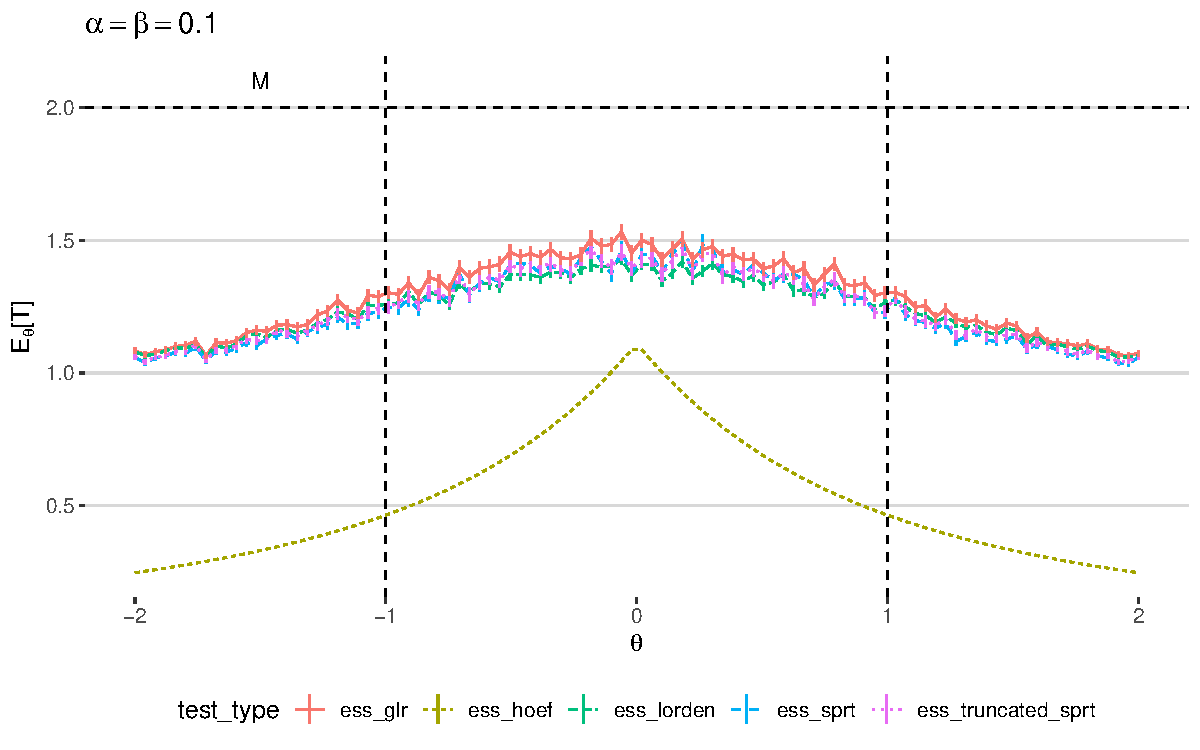
\includegraphics[width=\textwidth]{images/ess_alpha1e1}
\end{subfigure}
\hfill
\begin{subfigure}{0.49\textwidth}
    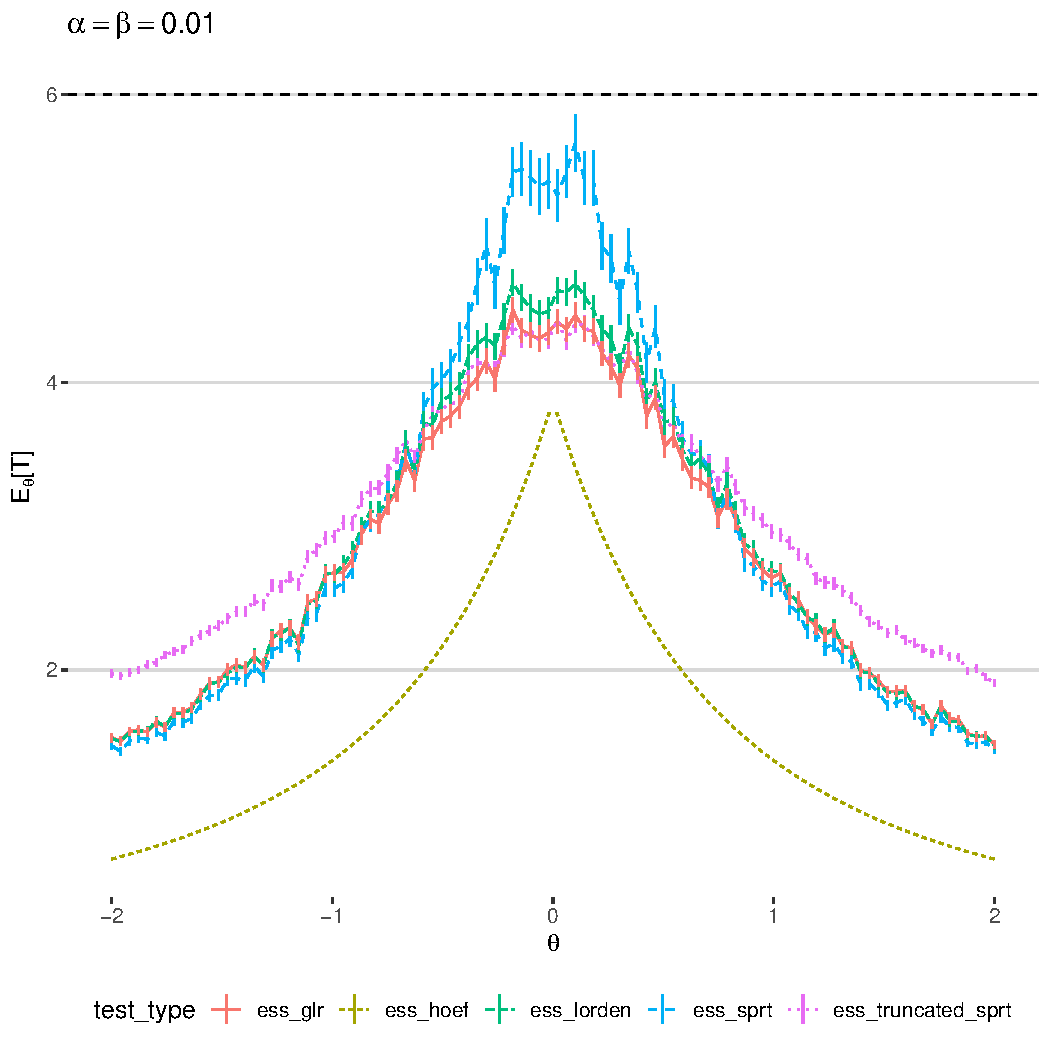
\includegraphics[width=\textwidth]{images/ess_alpha1e2}
\end{subfigure}
\begin{subfigure}{0.49\textwidth}
    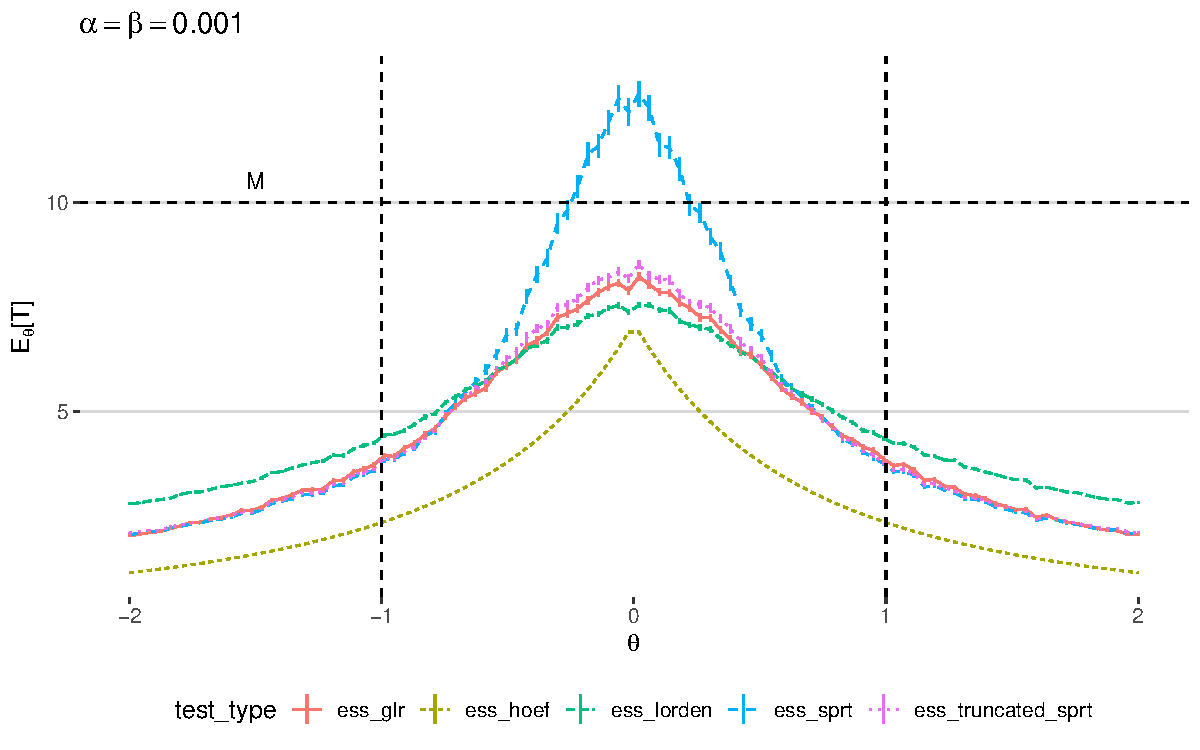
\includegraphics[width=\textwidth]{images/ess_alpha1e3}
\end{subfigure}
\hfill
\begin{subfigure}{0.49\textwidth}
    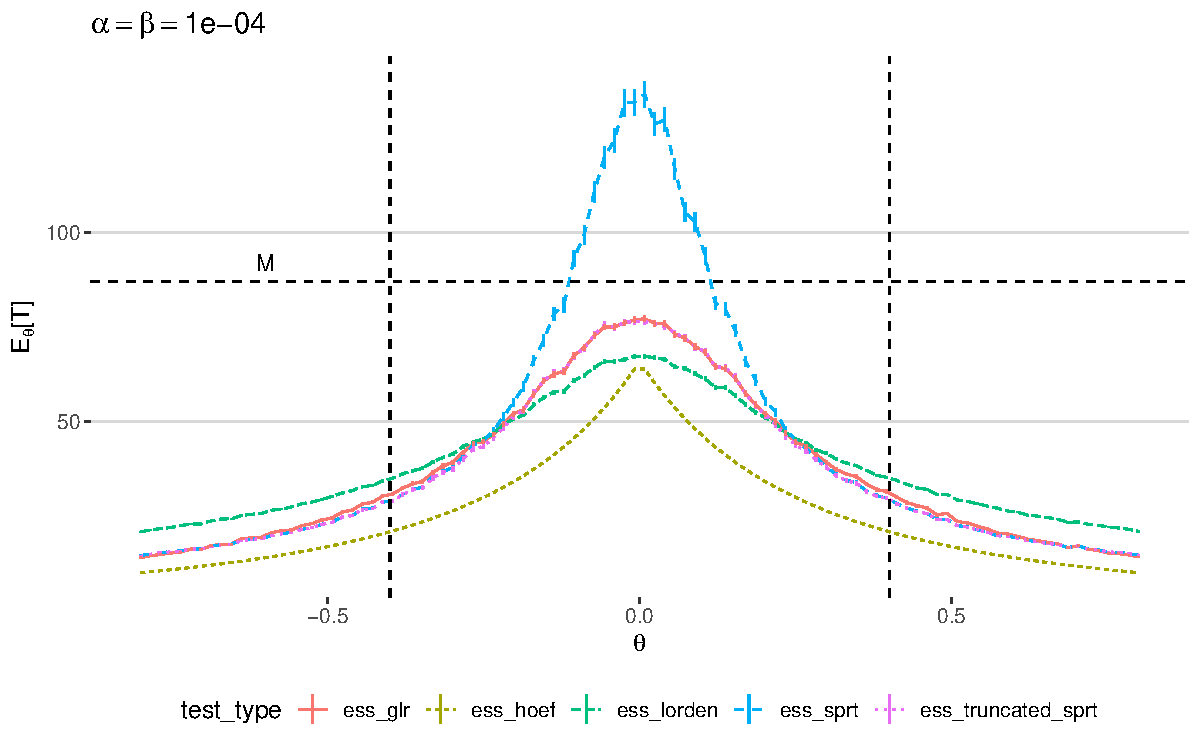
\includegraphics[width=\textwidth]{images/ess_alpha1e4}
\end{subfigure}

\caption{Comparison for the SPRT, Truncated SPRT, Lorden's 2-SPRT, and the GLR test when $X_i \overset{\text{iid}}\sim N(\theta, 1)$, $\theta_0 = -\theta_1 = 1$, and thresholds are choosen such that the error probabilities are $\alpha = \beta = 0.1, 10^{-2}, 10^{-3}, 10^{-4}$. The mixing proportion was set to $c_1 = c_2 = 0.5$ for the Truncated SPRT. For large error probabilities (0.1 or $10^{-2}$, the Truncated SPRT generally performs worse or equivalent to Lorden's 2-SPRT and the GLR test. For small error probabilities, the Truncated SPRT has uniformly lower ESS between 0.5 and $-0.5$, but has much heavy tails for large $\theta$. All tests besides the SPRT have a smaller sample size on average than the equivalent FSS test.}
\end{figure}

\section{Conclusion}

\newpage
\bibliographystyle{asa}
\bibliography{reference}

\end{document}
